\hspace{24pt}
% \renewcommand{\baselinestretch}{1.5}

This paper attempts to improve prediction of cell line-specific cases by utilizing DNA methylation signal, and introduce an inception module into the CNN to increase the ability to extract features. In our problem formulation, we define prediction of six histone modifications in a window as a binary classification task, given a fixed-length segment of DNA sequence and methylation signal. This is known as a multi-label classification task, where multiple labels can be positive at once.

\begin{figure}[H]
    \centering
    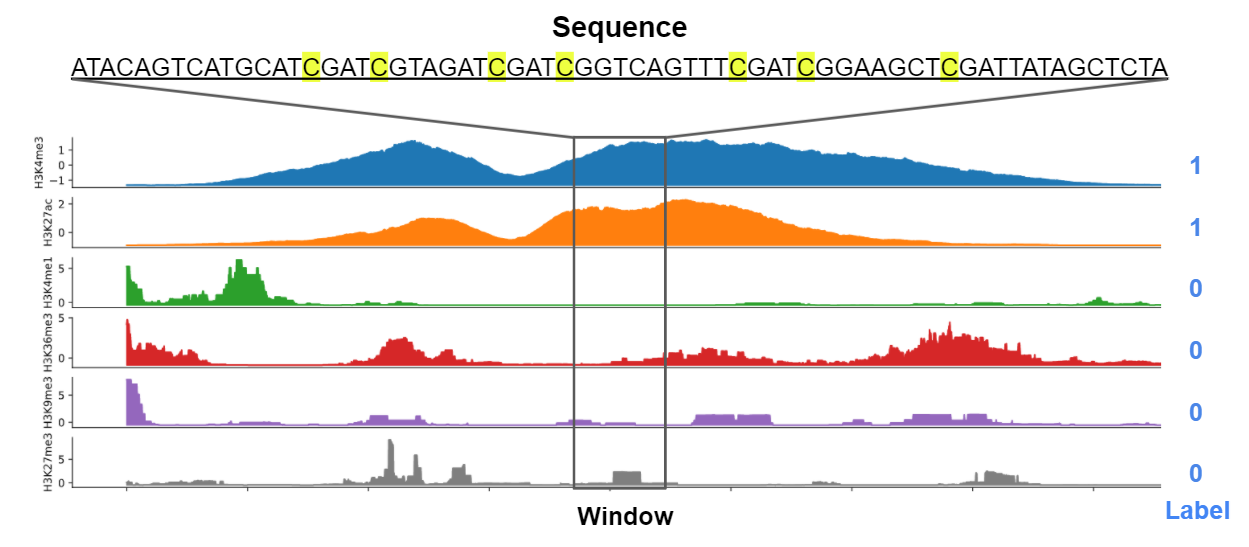
\includegraphics[width=1\columnwidth]{body/figure/figure3.png}
    \captionsetup{labelfont=bf}
    \renewcommand{\baselinestretch}{1.0}
    \caption[Pair of input and label]{The methylated cytosines are marked by yellow in DNA sequence.}
    \label{f3}
\end{figure}

\section{Data Preprocessing}
We download peak files of six histone modifications for three human epigenomes from the ENCODE project. These six histone modifications, including H3K4me1, H3K4me3, H3K9me3, H3K27ac, H3K27me3 and H3K36me3, are important markers that have been verified to be associated with specific functional regions in the genome, as shown in Table~\ref{t1}. For convenience and efficient experiment, we first select 3 epigenomes in the category of cell lines, which have complete dataset that six histone modifications and methylation signal. There are including A549, GM12878 and K562, where GM12878 and K562 are widely used in ENCODE and Roadmap project \cite{davis2018encyclopedia}\cite{kundaje2015integrative}.

Peak file is generated by peak calling algorithm, which is a step of standard pipeline of capturing protein-binding regions. This file indicates where is binding regions, called peak, in genome, and the signal value of binding regions. Given six peak files of each cell lines, we use a window of 200bp to scan the whole human genome with step 200 bp, and regard a window that has at least 100 bp overlap with peak as a histone modification binding site, shown in Figure~\ref{f3}. Our setting is similar to DeepHistone \cite{yin2019deephistone}, but we add additional rule that at least one positive peak in window. Because most of peaks of any histone modifications in genome is not active and not interesting to us, we add this rule to remove lots of windows, whose all labels are negative.

\begin{table}[H]%加入table環境指令以控制表格的位置、編號與標題,[h]代表將表格置於here,其他位置的標示請參考手冊
    \centering
    \begin{tabular}{lcccc}
    \hline
        Cell line & A549 & M12878 & K562	 \\\hline
        H3K4me3 & 163727 (0.06) & 253760 (0.32) & 154500 (0.1) \\
        H3K27ac & 697041 (0.23) & 294976 (0.37) & 227165 (0.14) \\
        H3K4me1 & 537240 (0.18) & 355490 (0.44) & 520504 (0.34) \\
        H3K36me3 & 1068720 (0.36) & 140428 (0.17) & 129438 (0.08) \\
        H3K9me3 & 223102 (0.08) & 63791 (0.08) & 51017 (0.03) \\
        H3K27me3 & 1000516 (0.34) & 63640 (0.08) & 745326 (0.49) \\\hline
        Total & 2961825 & 805361 & 1521904\\\hline
    \end{tabular}
    \captionsetup{labelfont=bf}
    \renewcommand{\baselinestretch}{1.0}
    \caption[Amount of windows of each cell line]{These entries are amount of positive peak of six histone modification in each cell line. The bottom row represents total number of windows.The number in the parenthesis is percentage of positive peak in each histone modification.}
    \label{t3}
\end{table}

We then download the human reference genome (GRCh38) and extract the 2000bp DNA sequence surrounding the center of each window as an input, since the motif for a special signal is may not be contained in the 1000bp \cite{lanchantin2020graph}, whereas DeepSEA, DanQ and DeepHistone set 1000bp. Next, we covert base of DNA sequence to value, and combine methylation signal into input matrix. These are separately encoded by one-hot encoding scheme, as well as positive-stranded and negative-stranded methylation percentage. As a result, the input of model is a 5 * 2000 matrix, including features from four bases and methylation.

After creating the pair of input features and label, we first divide each dataset of each cell line into ten partitions because whole dataset can not be stored in memory. To obtain more representative partition of dataset, we use stratified sampling to split against labels so that each partition of dataset has same distribution.

\section{Convolutional neural network on sequence data}
Convolutional neural network (CNN) is one of the most popular algorithms in deep-learning field. CNN has been successfully applied on many applications. Especially, it makes a lot of progress in image recognition, because shared weights and local connections in the CNN are employed to make full use of 2D input-data structures \cite{alzubaidi2021review}.

CNN is mainly composed of convolutional layer, pooling layer and fully connected layer. First, convolutional layer is a group of convolutional filters, also called kernels. Each kernel scan input data to extract local features with convolutional operation, and generate output called feature map \cite{alzubaidi2021review}. According to above description, we can apparently observe the property of convolutional layer that modeling invariant features. This allows CNNs effectively learn correct “motifs” from DNA sequences, that the patterns is learned by kernel. The diagram of convolutional layer is shown on following Figure~\ref{f4}.

\begin{figure}[H]
    \centering
    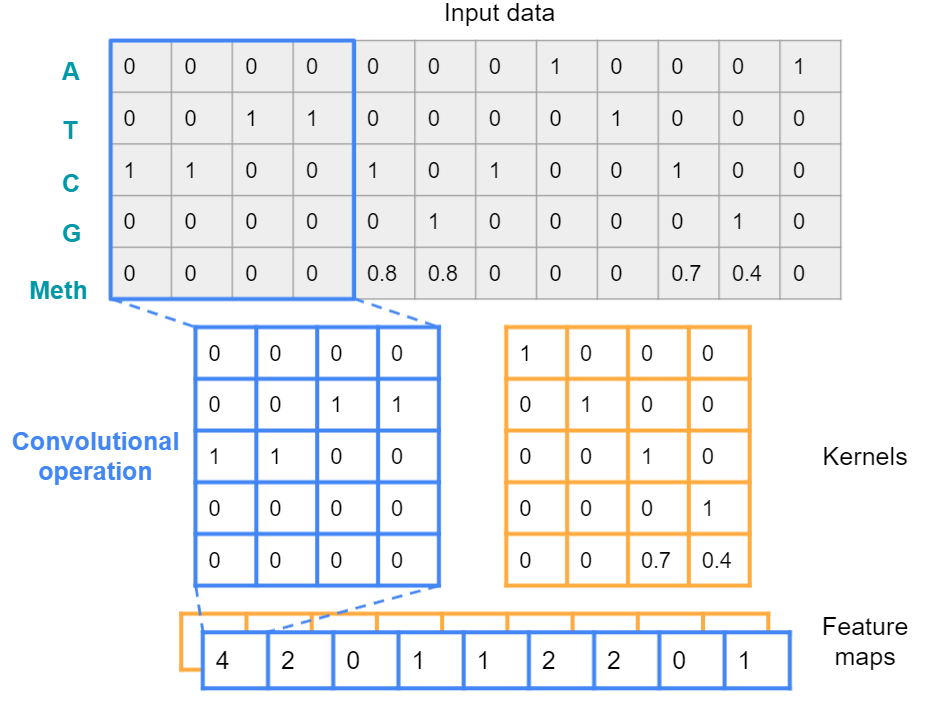
\includegraphics[width=1\columnwidth]{body/figure/figure4.png}
    \captionsetup{labelfont=bf}
    \renewcommand{\baselinestretch}{1.0}
    \caption[Convolutional operation]{Convolutional operation is that element-wised multiplication, and then summation. Parameters in kernels are like neuron in network, that is learned.}
    \label{f4}
\end{figure}

Second, pooling layer is that sampling the feature maps generated by convolutional layers. The main goal is to shrink feature maps, without lose important information. There are several types of pooling methods implemented in pooling layers, including max pooling, average pooling, and so on \cite{alzubaidi2021review}. The most common pooling layer is max pooling, shown in following Figure~\ref{f5}.

\begin{figure}[H]
    \centering
    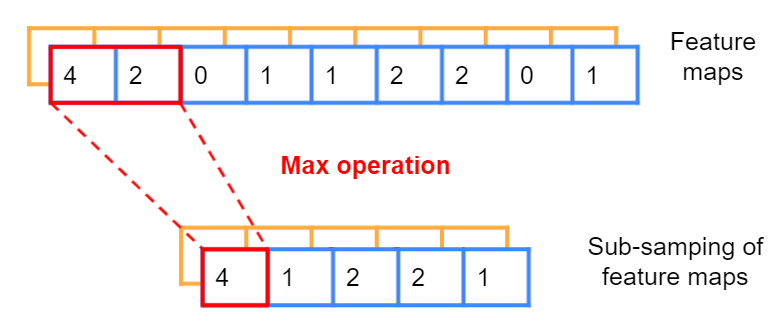
\includegraphics[width=0.9\columnwidth]{body/figure/figure5.png}
    \captionsetup{labelfont=bf}
    \renewcommand{\baselinestretch}{1.0}
    \caption[Operation of max pooling]{Pooling layer is similar to convolutional layer. It calculates within small region, also called kernel, and output one value in feature map.}
    \label{f5}
\end{figure}

Third, fully connected layer is often located on end of CNN and acts as classifier. Its input is the feature extracted by previous convolutional layers and pooling layers. Because input of fully connected layer is in the form of a vector, feature maps should be flatten as a vector \cite{alzubaidi2021review}. Then, the classifier takes feature vector to predict.

\begin{figure}[H]
    \centering
    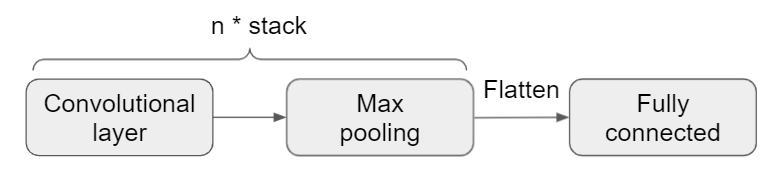
\includegraphics[width=0.9\columnwidth]{body/figure/figure6.png}
    \captionsetup{labelfont=bf}
    \renewcommand{\baselinestretch}{1.0}
    \caption[Standard pipeline of convolutional neural network]{Standard pipeline of convolutional neural network.}
    \label{f6}
\end{figure}

Figure~\ref{f6} is standard pipeline in CNN, which extracts features through convolutional layers and pooling layers, and then classifies through fully connected layers. Convolutional layers and pooling layers can be stacked many times to increase capability of CNN. Although there are many variants of CNN, main pipeline like Figure~\ref{f6} is not changed.

\section{Inception Module}
The trend in deep learning is that utilizing deeper and wider architectures to improve quality of networks. In 2014, Szegedy et al. introduce inception module into GoogLeNet. Inception module is designed by different kernel sizes to extract various scale features, shown in Figure~\ref{f7}. It makes model wider and gets better performance \cite{szegedy2015going}.

\begin{figure}[H]
    \centering
    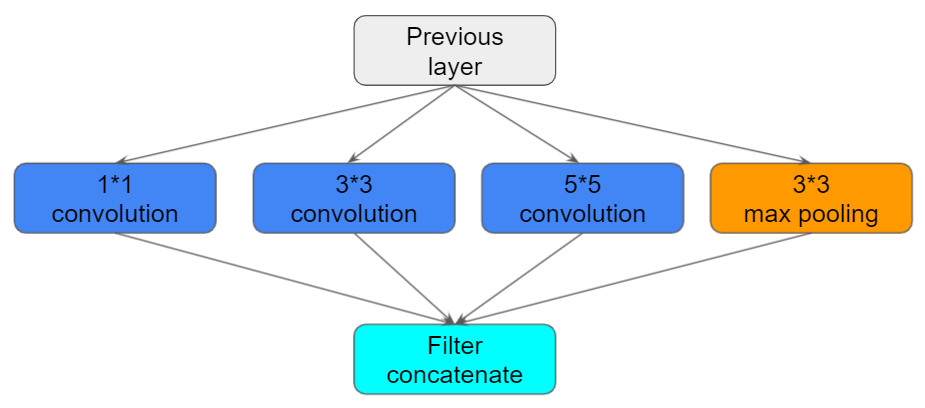
\includegraphics[width=0.8\columnwidth]{body/figure/figure7.png}
    \captionsetup{labelfont=bf}
    \renewcommand{\baselinestretch}{1.0}
    \caption[Naive version of inception module]{Naive version of inception module.}
    \label{f7}
\end{figure}

But, the complex model is readily to overfitting, and is not easily trained on limited computational source. This common problem has existed in model-based method for a long time. Accordingly, to overcome this problem, Szegedy et al. add two methods into model, 1 * 1 convolutional layer and global average pooling. First, 1 * 1 convolutional layer is just a convolutional layer whose kernel size is one. When it is added on top of convolutional layer, it can learn more non-linear information from previous layer, and effectively scale the dimensions of feature maps to reduce calculation in model, shown in Figure~\ref{f8} \cite{lin2013network}. Second, global average pooling is a kind of average pooling, whose kernel size is equal to size of feature map. This mechanism is located at the last pooling layer, to reduce parameters of connection between feature maps and fully connected layer \cite{lin2013network}. Hence, GoogLeNet is allowed for increasing the depth and width of the network, while keeping the computational budget constant. Also, GoogLeNet won the ImageNet Large-Scale Visual Recognition Challenge (ILSVRC) in 2014.

\begin{figure}[H]
    \centering
    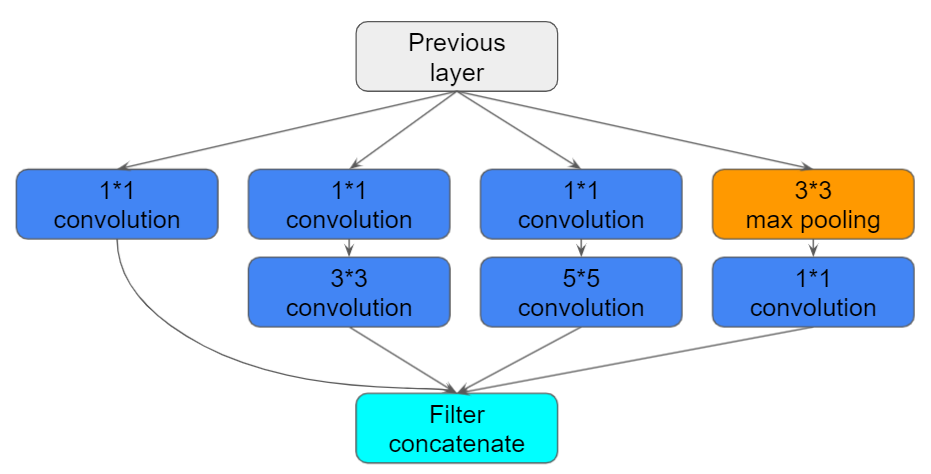
\includegraphics[width=0.8\columnwidth]{body/figure/figure8.png}
    \captionsetup{labelfont=bf}
    \renewcommand{\baselinestretch}{1.0}
    \caption[Final version of inception module]{Final version of inception module, implemented in GoogLeNet.}
    \label{f8}
\end{figure}

\section{Model Architecture} \label{method}
We select the convolutional neural network as our framework, which consists of multiple convolutional layers, pooling layers and fully connected layers, because convolutional layer is good at extracting motifs in genome. In addition, we add inception module into our model so that extract more representative features through kernels of different scales. The complete architecture is depicted in Figure~\ref{f12}, where detailed modules are used in Figure~\ref{f9}. The details of the structure are explained and summarized as follows:

\begin{figure}[H]
    \centering
    \subfigure[Input layer]{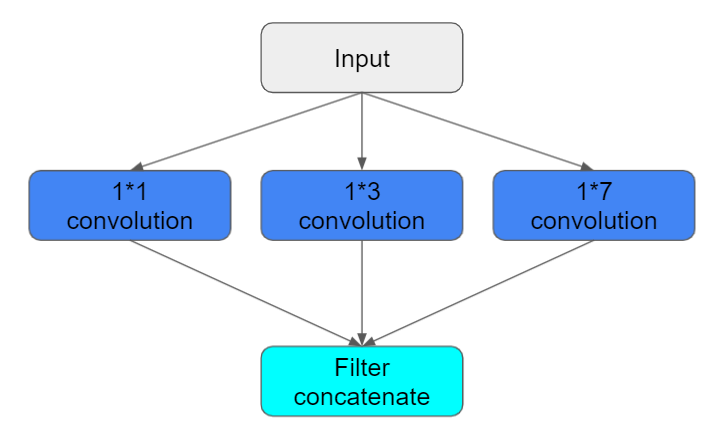
\includegraphics[width=0.65\columnwidth]{body/figure/figure9.png}}\\
    \centering
    \subfigure[Inception module-a]{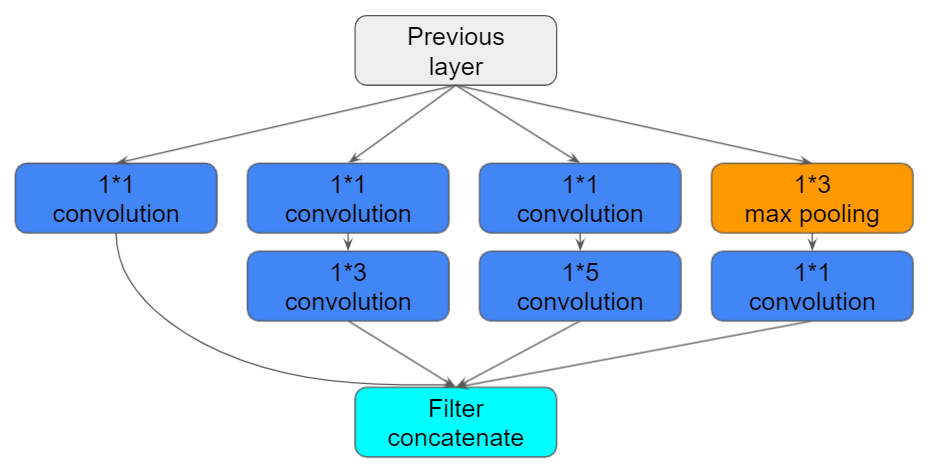
\includegraphics[width=0.75\columnwidth]{body/figure/figure10.png}}\\
    \centering
    \subfigure[Inception module-b]{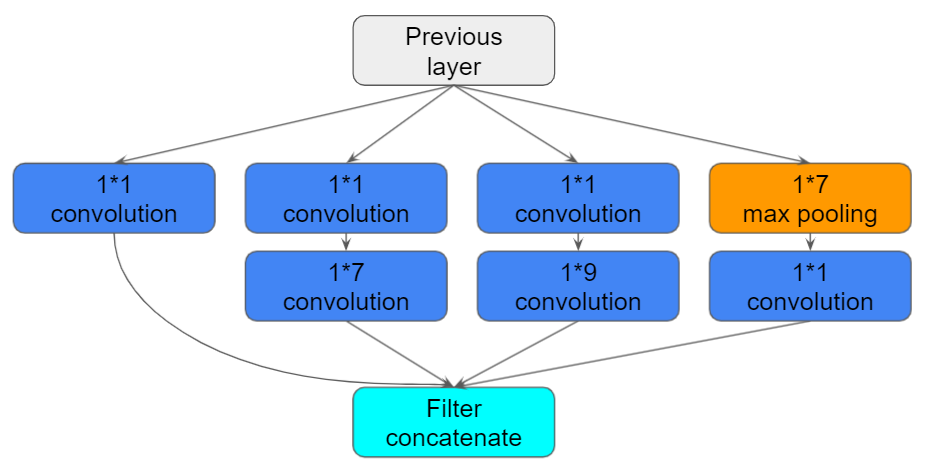
\includegraphics[width=0.75\columnwidth]{body/figure/figure11.png}}\\
    \captionsetup{labelfont=bf}
    \renewcommand{\baselinestretch}{1.0}
    \caption[Structure of detailed modules]{Inception module-b. 1 * n means that length n of sequence of extracting features at once.  The block of filter concatenate in all figures is to stack all feature maps from each branch together.}
    \label{f9}
\end{figure}

In terms of convolutional layer, we remove bias of all convolutional layers because of reducing parameters of model. It can not only avoid model too complex but increase batch size. Next, the outputs of all convolutional layers are orderly passed through the batch normalization layer and rectified linear unit (ReLU). They are respectively for avoiding overfitting and activation.

In terms of pooling layer, all max pooling layers of kernel size are three, and step with two. The goal of these layers is to sample the feature maps from previous layer, and reduce the length of feature map. After passing last pooling layer, one dropout layer with fifty percentage of dropped outputs was performed in training.

In terms of fully connected layers, they are located at the end of stacked convolutional layers and pooling layers, to predict histone modifications. We design two fully connected layers, individually 100 neurons and 6 neurons.

\begin{figure}[H]
    \centering
    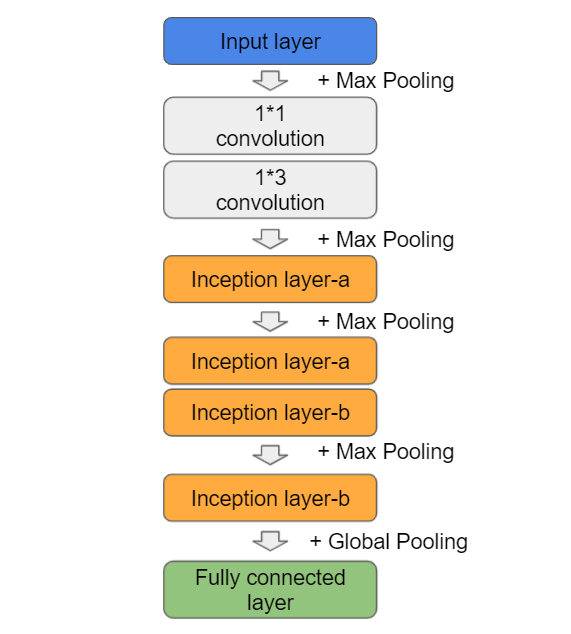
\includegraphics[width=0.7\columnwidth]{body/figure/figure12.png}
    \captionsetup{labelfont=bf}
    \renewcommand{\baselinestretch}{1.0}
    \caption[Complete architecture]{The overall architecture of our model. Global pooling represents global average pooling, located on top of the block of fully connected layer.}
    \label{f12}
\end{figure}

In terms of training methodology, our model is trained using stochastic gradient descent with momentum of 0.9, a learning rate of 0.01, and trained using a batch size of 300. For our loss function, we use the mean binary cross-entropy with sigmoid function \(\sigma\) across all labels $L$, shown in equation~\ref{eq:weight}.  In equation~\ref{eq:weight}, $w_\ell$ is the weight to scale the given to the loss of each positive element. It can deal with imbalance status in each class. According to Table~\ref{t3}, our dataset is imbalanced in class distribution. Hence, we set the weights inversely proportional to percentage of positive peaks for each histone modification, to mitigate the effects of this imbalance.

%%\[  F(y, \hat{y}) = \frac{1}{L}\sum_{l=1}^{L}-(w_l*y_i^llog\sigma(\hat{y}_i^l)+(1-y_i^l)log(1- \sigma(\hat{y}_i^l) ))\ \ (1)  \]

\begin{equation}
F(y, \hat{y}) = \frac{-1}{L}\sum_{\ell=1}^{L} \left( w_\ell\,y_i^\ell\log\sigma(\hat{y}_i^\ell) \,+\, (1-y_i^\ell)\log(1-\sigma \hat{y}_i^\ell) \right)
\label{eq:weight}
\end{equation}

\section{Stratified mini-batch}
However, only setting the weight in loss function is not enough to deal with imbalanced multi-label tasks, as shown in Section~\ref{strat}. Imbalanced learning is still a challenging issue because model-based methods for any task are significantly affected by skewed datasets \cite{buda2018systematic}. In order to obtain higher accuracy, the classifier tends to ignore labels with low frequency, which lead to more errors in minority classes. Therefore, Peng et al.\ propose the method, that introduce stratified sampling to modify the sampling operation of mini-batch learning, to solve this issue \cite{peng2021addressing}. In this paper, Peng et al.\ designed the two stratified sampling against label powerset and label. Label powerset-based stratification is that sampling dataset according to the distribution of all label combinations. But, this stratification select samples from a large number of labels combinations, resulting in the construction of a large mini-batch that is not suitable for the training of the model. Label-based stratification is that sampling dataset according to the distribution of all label classes. Compared to label powerset-based stratification, it only considers the number of label classes, that fewer number of stratifications is good for our limited computational resource. Accordingly, we introduce the label-based stratified sampling into mini-batch learning, to keep the distribution of each mini-batch the same as the whole dataset.
